% !TeX encoding = UTF-8

%% ------------------------------------------------------------------------
%% Copyright (C) 2021 SJTUG
%% 
%% SJTUBeamer Example Document by SJTUG
%% 
%% SJTUBeamer Example Document is licensed under a
%% Creative Commons Attribution-NonCommercial-ShareAlike 4.0 International License.
%% 
%% You should have received a copy of the license along with this
%% work. If not, see <http://creativecommons.org/licenses/by-nc-sa/4.0/>.
%% -----------------------------------------------------------------------

\documentclass[xcolor=table,dvipsnames,svgnames,aspectratio=169]{ctexbeamer}
% 可以通过 fontset=macnew / fontset=ubuntu / fontset=windows 选项切换字体集

\usepackage{tikz}
\usepackage[normalem]{ulem}
\usetikzlibrary{arrows}
\usepackage{amsmath}
\usepackage{mflogo}
\usepackage{graphicx}
\usepackage{xspace}
\usepackage{amsmath}
\usepackage{unicode-math}
\usepackage{ccicons}
\usepackage{hologo}
\usepackage{colortbl}
\usepackage{shapepar}
\usepackage{hyperxmp}
\usepackage{booktabs}
\usepackage{qrcode}
\usepackage{listings}
\usepackage{tipa}
\usepackage{multicol}
\usepackage{datetime2}
\usepackage{fontawesome5}
\usepackage{hyperref}
\usepackage[backend=biber,style=gb7714-2015]{biblatex}

\addbibresource{thesis.bib}
\setbeamertemplate{bibliography item}[text]

\graphicspath{{figures/}}

\hypersetup{
  pdfsubject = {上海交通大学图书馆专题培训讲座},
  pdfauthor = {Alexara Wu},
  pdfcopyright = {Licensed under CC-BY-SA 4.0. Some rights reserved.},
  pdflicenseurl = {http://creativecommons.org/licenses/by-sa/4.0/},
  unicode            = true,
  psdextra           = true,
  pdfdisplaydoctitle = true
}

\pdfstringdefDisableCommands{
  \let\\\relax
  \let\quad\relax
  \let\hspace\@gobble
}

\renewcommand{\TeX}{\hologo{TeX}}
\renewcommand{\LaTeX}{\hologo{LaTeX}}
\newcommand{\BibTeX}{\hologo{BibTeX}}
\newcommand{\XeTeX}{\hologo{XeTeX}}
\newcommand{\pdfTeX}{\hologo{pdfTeX}}
\newcommand{\LuaTeX}{\hologo{LuaTeX}}
\renewcommand{\CTeX}{C\TeX}
\newcommand{\MiKTeX}{\hologo{MiKTeX}}
\newcommand{\MacTeX}{Mac\hologo{TeX}}
\newcommand{\beamer}{\textsc{beamer}}
\newcommand{\XeLaTeX}{\hologo{Xe}\kern-.13em\LaTeX{}}
\newcommand{\pdfLaTeX}{pdf\LaTeX{}}
\newcommand{\LuaLaTeX}{Lua\LaTeX{}}

\def\TeXLive{\TeX{} Live\xspace}
\let\TL=\TeXLive
\newcommand{\SJTUThesis}{\textsc{SJTUThesis}\xspace}
\newcommand{\SJTUBeamer}{\textsc{SJTUBeamer}\xspace}
\newcommand{\SJTUThesisVersion}{1.0.0rc7}
\newcommand{\SJTUThesisDate}{2020/7/31}

\newcommand\link[1]{\href{#1}{\faLink}}
\newcommand\pkg[1]{\texttt{#1}}

\def\cmd#1{\texttt{\color{DarkBlue}\footnotesize $\backslash$#1}}
\def\env#1{\texttt{\color{DarkBlue}\footnotesize #1}}
\def\cmdxmp#1#2#3{\small{\texttt{\color{DarkBlue}$\backslash$#1}\{#2\}\hspace{1em}\\ $\Rightarrow$\hspace{1em} {#3}\par\vskip1em}}

\lstset{
  language=[LaTeX]TeX,
  basicstyle=\ttfamily\footnotesize,
  tabsize=2,
  keywordstyle=\bfseries\ttfamily\color{cprimary},
  commentstyle=\sl\ttfamily\color[RGB]{100,100,100},
  stringstyle=\ttfamily\color[RGB]{50,50,50},
  extendedchars=true,
  breaklines=true,
}

\lstdefinestyle{style@inline}{
  basicstyle   = \ttfamily,
  keepspaces   = true
}
\lstMakeShortInline[style=style@inline]|

\usetheme[maxplus]{sjtubeamer}
% 使用 maxplus/max/min 切换标题页样式
% 使用 red/blue 切换主色调
% 使用 light/dark 切换亮/暗色模式
% 使用外样式关键词以获得不同的边栏样式
%   miniframes infolines  sidebar* 
%   default    smoothbars split	 
%   shadow     tree       smoothtree
% *siderbar 推荐与 max 一起使用。

% \tikzexternalize[prefix=cache/]
% 如果您需要缓存 tikz 图像,请取消注释上一行,并在编译选项中添加 -shell-escape。

\author{Alexara Wu}
\institute[SJTUG]{上海交通大学 Linux 用户组}
\date{\the\year 年 \the\month 月}
\subject{LaTeX, 论文排版, SJTUThesis}

\title[\SJTUBeamer 示例文档] % 页脚显示标题
{\textbf{如何使用 \LaTeX 排版论文}} % 首页标题

\subtitle{\SJTUBeamer 示例文档}

\begin{document}

% 使用节目录
\AtBeginSection[]{
  \begin{frame}
    % \tableofcontents[currentsection]           % 传统节目录             
    \sectionpage                   % 节页
  \end{frame}
}

% 使用小节目录
\AtBeginSubsection[]{                  % 在每小节开始
  \begin{frame}
    % \tableofcontents[currentsection,currentsubsection]             % 传统小节目录             
    \subsectionpage                % 小节页
  \end{frame}
}

\maketitle

\begin{frame}{目录}
  \tableofcontents
\end{frame}

% !TeX encoding = UTF-8
% !TeX root = ../main.tex

%% ------------------------------------------------------------------------
%% Copyright (C) 2021 SJTUG
%% 
%% SJTUBeamer Example Document by SJTUG
%% 
%% SJTUBeamer Example Document is licensed under a
%% Creative Commons Attribution-NonCommercial-ShareAlike 4.0 International License.
%% 
%% You should have received a copy of the license along with this
%% work. If not, see <http://creativecommons.org/licenses/by-nc-sa/4.0/>.
%% -----------------------------------------------------------------------

\section{Introduction}

\subsection{Background}

%\begin{frame}{Motivation}
%  Reasons behind my research paper choice:
%  \begin{itemize}
%    \item My research line is mainly targeted to blockchain technology
%    \item This specific research paper has been developed by my PhD co-supervisors (good chance to learn about their researching style)
%    \item My PhD thesis could use some of the model simulation techniques (stochastic processes) used in this research paper experimentation
%    \item And of course, it is related to a emerging subfield that could greatly contribute to the development of the Internet of Things (IoT)
%  \end{itemize}
%\end{frame}

\begin{frame}[fragile]{Background}

  Blockchain technology $\rightarrow$ theoretical potential:
  \begin{itemize}
		\item Data integrity
		\item Decentralizing trust
		\item Reducing costs
  \end{itemize}
	
  Useful practical application? $\rightarrow$ \alert{e-government} (software administration processes)
    
   \begin{exampleblock}{From generic case to more specific}
    	\textbf{studenty mobility management} $\subset$ supply chain management
  \end{exampleblock}

\end{frame}

%\subsection{Crowdsensing}
%
%\begin{frame}{Crowdsensing: definition}
%  \begin{itemize}
%  \item \textbf{Crowdsensing:} emerging paradigm of data aggregation\cite{paper1}, having a key role in data-driven applications. Specially used for getting large ammounts of IoT sensing data, by using the individual intelligent sensing devices.
%  \item \textbf{Benefit:} improved data collection efficiency and reduced costs effectively\cite{paper2}
%  \end{itemize}
%  \begin{figure}[h]
%        \centering
%        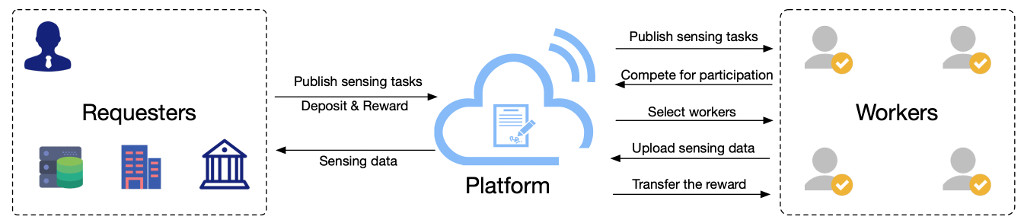
\includegraphics[width=.8\textwidth]{201909-wei-figure1.jpg}
%      \end{figure}
%\end{frame}
%
%\begin{frame}{Crowdsensing: issues}
%  		\begin{enumerate}
%   			\item Managed and maintained \alert{centralized platforms} suffer from the single point of failure
%   				\begin{itemize}
%   					\item \textbf{Proposal: } decentralized architecture (blockchain technology) that lacks a single point of failure, and enhances privacy with asymmetric encryption and digital signature technology
%   				\end{itemize}
%    		\item Encouraging workers by offering appropiate \alert{incentive mechanisms} (monetary usually) \rightarrow  \underline{auction theory} guarantees benefits for both requesters and workers\cite{paper15} but only provide short-term incentives
%    			\begin{itemize}
%   					\item \textbf{Proposal:} hybrid incentive mechanism, adopting \underline{mechanism design theory}, considering three factors:
%   					\begin{itemize}
%   					\item Monetary reward
%   					\item Reputation evaluation
%   					\item Data quality
%   					\end{itemize}
%   				\end{itemize}
%  		\end{enumerate}
%\end{frame}

\include{contents/basis}
\include{contents/thesis}
\include{contents/summary}

\appendix

\begin{frame}
  \frametitle{参考文献}
  \printbibliography
\end{frame}

\makebottom

\end{document}
